\documentclass[12pt, letterpaper]{article}
\usepackage{graphicx} % Required for inserting images
\usepackage{hyperref}
\usepackage{listings}
\usepackage{amssymb}
\usepackage{amsmath}
\usepackage[english]{babel}
\usepackage{nicefrac, xfrac}
\usepackage{mathtools}
\newcommand{\acc}{\\\hphantom{}\\}
\usepackage[table,xcdraw]{xcolor}
\usepackage[paper=a4paper,left=20mm,right=20mm,bottom=25mm,top=25mm]{geometry}
\renewcommand{\labelenumii}{\arabic{enumi}.\arabic{enumii}}
    \renewcommand{\labelenumiii}{\arabic{enumi}.\arabic{enumii}.\arabic{enumiii}}
    \renewcommand{\labelenumiv}{\arabic{enumi}.\arabic{enumii}.\arabic{enumiii}.\arabic{enumiv}}
\title{Go (gruppo 42)}
% \author{ Giacomo Biribicchi \and Marco Casu \and Christian Di Manno \and Alessandro Gautieri }
\date{}


\begin{document}

\maketitle


\section{Requisiti}
I dati di interesse per il sistema sono \underline{Giocatori}, \underline{Tornei} e \underline{Partite}.
\begin{enumerate}
    \item \textbf{Giocatore}\begin{enumerate}
        \item nome
        \item cognome 
        \item nickname - il nickname univoco
        \item rank dichiarato - intero positivo
        \item indirizzo
    \end{enumerate}
    \item \textbf{Partita}\begin{enumerate}
        \item data - la data in cui si è disputata 
        \item luogo 
        \item regole - cinesi o giapponesi 
        \item giocatore pietre bianche 
        \item giocatore pietre nere 
        \item komi - fattore di decifit, $x\in[0,10]$
        \item esito - se ha vinto il bianco o il nero, rappresentato come rinuncia o coppia di punteggi
        \item eventuale torneo di riferimento
    \end{enumerate}
    \item \textbf{Torneo}\begin{enumerate}
        \item partite associate 
        \item nome 
        \item descrizione 
        \item edizione - anno in cui si svolge
    \end{enumerate}
\end{enumerate}
\newpage
\section{Considerazioni}

\section{Documenti di Specifica}
\subsection{Tipi di Dato}
Punteggio = \{b : Int$\ge$0, n : Int$\ge$0\}\acc 
Komi = \{Real $\in$ [0,10]\}\acc 
Regole = \{cinese,giapponese\}\acc
Rank = Int$\ge$0\acc 
Anno = ("19" or "20") concat ["00","99"]\{1\}\acc
Giocatore = \{bianco,nero\}
\section{UML}
\begin{center}
    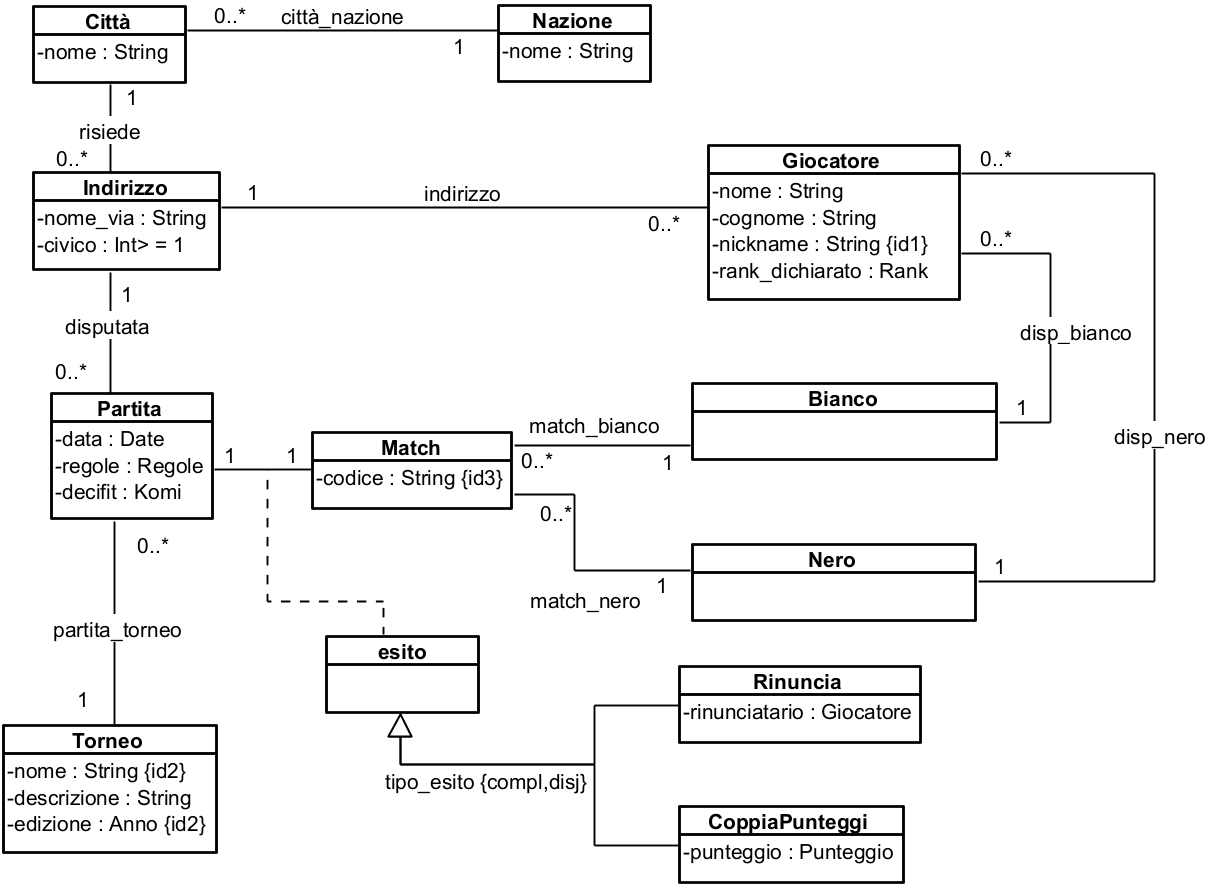
\includegraphics[width=\textwidth]{images/VPP.png}
\end{center}



\end{document}

